\documentclass{beamer}
\usetheme{metropolis}
\usepackage{graphicx}
\usepackage{tcolorbox}
\title{The Primer, Example Chapter: Appling an Integral}
\date{\today}
\author{Jordan Hanson}
\institute{Whittier College Department of Physics and Astronomy}

\begin{document}
\maketitle

\section{Contents}

\begin{frame}{Opening}
\begin{enumerate}
\small
\item \textbf{\alert{Symbolic Content}}: Depict idea through visual design
\item Confronting the Puzzle - Sum up a signal over time
\begin{itemize}
\item \textit{\alert{Classification}}: A problem involving an \textbf{integral}
\item \textit{\alert{Abstraction}}: Trade the \textbf{objects} for \textbf{symbols} and act on them
\item \textit{\alert{Hypothetical}}: Changing \textbf{properties} of symbols
\end{itemize}
\item Create an algorithm - one path
\begin{itemize}
\item \textit{Riemann sums} and \textit{pseudo-code}
\item \textbf{Testing}
\end{itemize}
\item Design a circuit - another path
\begin{itemize}
\item Translate symbols
\item \textbf{Build} and \textbf{Test}
\end{itemize}
\item \textbf{\alert{Study the mechanics result}}
\end{enumerate}
\end{frame}

\section{Confronting the Puzzle}

\begin{frame}{Confronting the Puzzle}
We encounter a \alert{signal}.  \textit{A bug walks across a magic pad (a sensor).  The pad gives only the current velocity of the bug.  We'd like to know how far the bug has traveled...} \\ 
\alert{\textbf{Symbolic content}}: Visual scene $\to$ \textit{\alert{Classification}} \\
\alert{\textbf{Symbolic content}}: Animate bug in scene $\to$ \textit{\alert{Classification}} \vspace{0.25cm}
\begin{tcolorbox}
Define \textbf{average velocity} and \textbf{displacement}: \\
\begin{align}
\vec{x} &= \vec{x}_{\rm f} - \vec{x}_{\rm i} \\
\vec{\bar{v}} &= \frac{\Delta \vec{x}}{\Delta t}
\end{align}
\end{tcolorbox}
\end{frame}

\begin{frame}{Confronting the Puzzle}
\alert{\textbf{Symbolic content}}: Observe that shrinking the time-window $\Delta t$ makes $\vec{v}$ more like the \textit{slope} of $\vec{x}(t)$, or the instantaneous velocity. \\ \vspace{0.5cm}
\begin{tcolorbox}
\textbf{Taking the limit}:
\begin{align} 
\lim_{\Delta t \to 0} \vec{\bar{v}} &= \vec{v}(t) = \frac{d\vec{x}}{dt} \\
\int_{0}^{x_{\rm 0}} \frac{dx}{dt} dt &= x_{\rm 0} \label{eq:eq1}
\end{align}
\end{tcolorbox}
\vspace{0.5cm}
\alert{\textbf{Symbolic content}}: Represent Eq. \ref{eq:eq1} visually $\to$ \textit{\alert{Abstraction}}
\end{frame}

\section{One path - Develop an Algorithm}

\begin{frame}{Develop an Algorithm}
\alert{\textbf{Symbolic content}}: \\ 
Breaking an integral into a: \textit{a Riemann sum} $\to$ \textit{\alert{Abstraction}} \vspace{0.5cm}
\begin{figure}
\centering
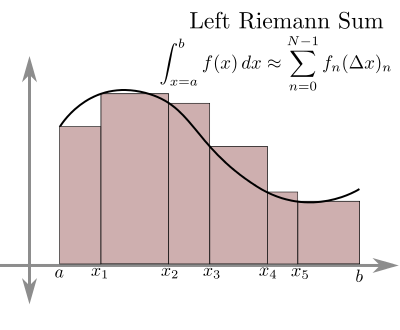
\includegraphics[width=0.4\textwidth]{figures/LeftRiemann.png}
\end{figure}
\begin{equation}
x_{\rm 0} = \sum_{n=0}^{N-1} f_n (\Delta x)_n
\end{equation}
\end{frame}

\begin{frame}[fragile]{Develop an Algorithm}
\begin{verbatim}
define x_0(t_data,v_data):
     delta_t = t_data[2]-t_data[1]
     x_0 = 0
     for i in v_data:
          x_0 += i*delta_t
     return x_0
\end{verbatim}
Study outputs given different data $\to$ \textit{\alert{hypothetical}}
\end{frame}

\section{Another Path - Design a Circuit}

\begin{frame}{Design a Circuit}
\begin{tcolorbox}
\textbf{Taking the limit}:
\begin{equation} 
\int_{0}^{x_{\rm 0}} \frac{dx}{dt} dt = x_{\rm 0}
\end{equation}
\end{tcolorbox}
\vspace{0.5cm}
\alert{\textbf{Symbolic content}}: Represent Eq. \ref{eq:eq1} visually $\to$ \textit{\alert{Classification}} \\
\begin{figure}
\centering
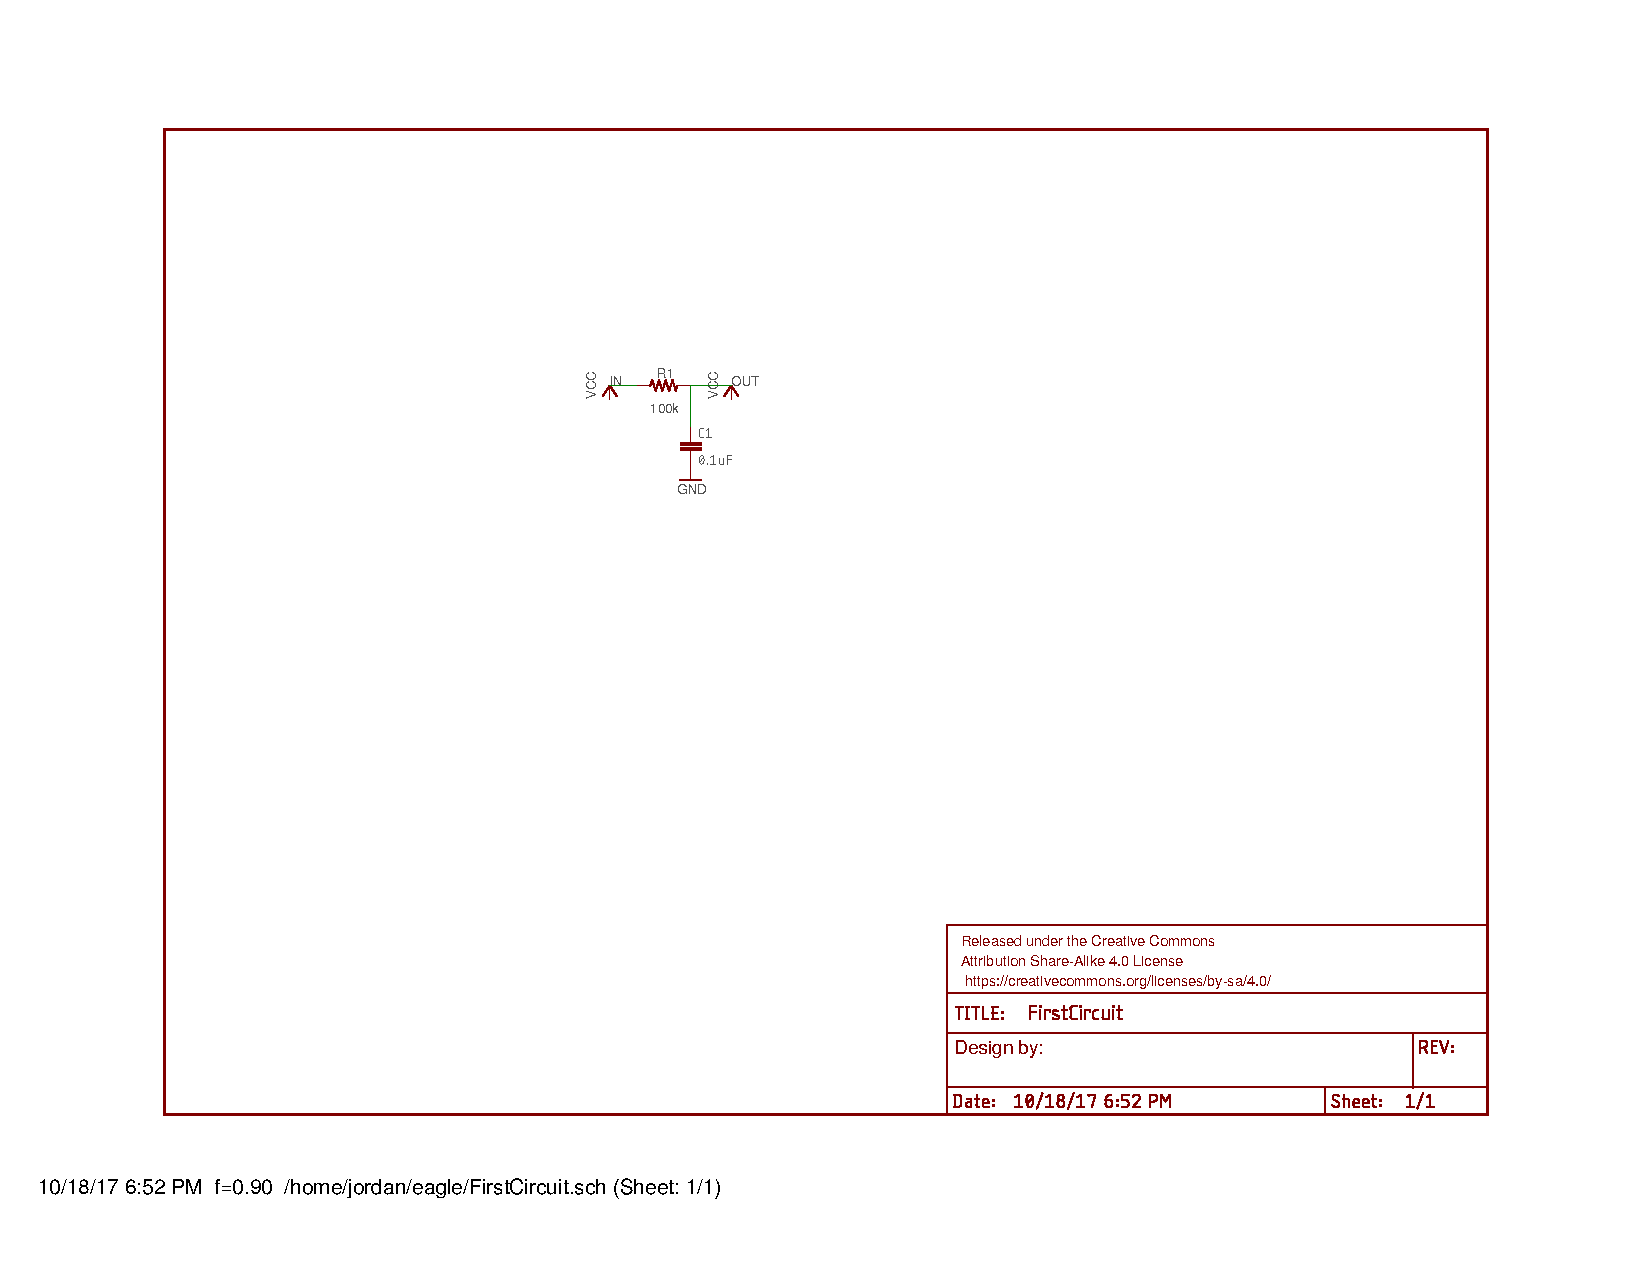
\includegraphics[width=0.5\textwidth,trim=9.5cm 13cm 15cm 6cm,clip=true]{figures/FirstCircuit.pdf}
\end{figure}
\end{frame}

\begin{frame}{Design a Circuit}
Show in steps that this circuit obeys $\to$ \textit{\alert{Abstraction}} \\
\begin{tcolorbox}
\begin{equation}
v_{\rm out} (t) = \frac{1}{RC} \int_{t_1}^{t_2} v_{\rm in}(t) dt
\end{equation}
\end{tcolorbox}
\begin{itemize}
\item See $v_{\rm out}(t)$ is like $x_{\rm 0}$, and $v_{\rm in}(t)$ is like $\vec{v}(t)$ $\to$ \textit{\alert{Classification}}
\item \textit{Build the circuit} (hypothetically in the book) $\to$ \textit{\alert{Abstraction}}
\item \textit{Test the circuit} for different outputs $\to$ \textit{\alert{Hypothetical}}
\end{itemize}
\alert{\textbf{Symbolic content}}: Show circuit and graph inputs and outputs
\end{frame}

\section{Study the Mechanics Result}

\begin{frame}{Study the Mechanics Result}
Using both or either paths (\textbf{Scalar}), solve the problem of $x_{\rm 0}$ using the content $\to$ \textit{\alert{Hypothetical}}
\begin{itemize}
\item Solution for the case of no motion
\item Solution for the case of constant velocity
\item Solution for the case of constant acceleration
\end{itemize}
\alert{\textbf{Symbolic content}}: Show these solutions graphically \\
$\to$ \textit{\alert{Abstraction}} (\alert{\textbf{Symbolic content}}): Deduce equations for displacement, given each situation
\end{frame}

\begin{frame}{Study the Mechanics Result}
Arrive at the answers: \\
\begin{align}
x_{\rm 0} &= x_{\rm i} \\
x_{\rm 0} &= vt + x_{\rm i} \\
x_{\rm 0} &= \frac{1}{2}at^2 + vt + x_{\rm i} 
\end{align}
\end{frame}

\section{Conclusion}

\begin{frame}{Conclusion}
\begin{enumerate}
\small
\item Confronting the Puzzle - Sum up a signal over time
\item Create an algorithm - one path
\item Design a circuit - another path
\item \textbf{\alert{Study the mechanics result}}
\end{enumerate}
\end{frame}

\end{document}
